\subsection{Radon profile classification}
\label{sec:Radon-classification}

\cite{2018MNRAS.480.2217S} identified 5 commonly recurring patterns in the stellar and gas Radon profiles of their MaNGA sample. These patterns were used to classify the Radon profiles observed in their MaNGA sample. In this work we adopt the same classification approach for the Radon profiles of the PSB galaxies and their control samples. Simplified models of 4 of the classes are shown in Figure \ref{fig:class-models}. In addition an asymmetric profile class was identified. The salient features of the Radon profile classes are listed below:

\begin{itemize}
    \item Constant, \textbf{Type-C} : Radon profile with relatively constant trace minimum angle $\hat{\theta}$ at all radii $\rho$.
    \item Inner Bend, \textbf{Type-IB} : Galaxies whose Radon profiles exhibit symmetrical variations of $\hat{\theta}$ beginning at $|\rho|=0$, then transitioning to a constant value. 
    \item Outer Bend, \textbf{Type-OB} : Galaxies with constant Radon trace angle $\hat{\theta}$  at small $|\rho|$ which transition to a different value at a greater radius. 
    \item Inner Bend + Outer Bend, \textbf{Type-IB+OB} : Galaxies with Radon profiles showing a combination of the features of Type-IB and Type OB profiles.
    \item Asymmetric, \textbf{Type-A} : The value of the $\hat{\theta}$ varies significantly with $\rho$ across opposite sides of the transform R\textsubscript{AB}. 
 \end{itemize}

\begin{figure}
    \centering
    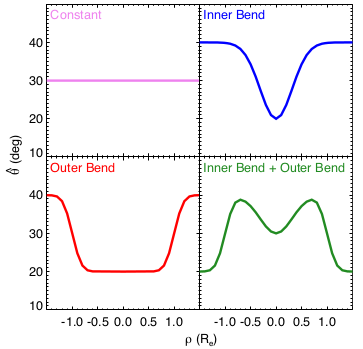
\includegraphics[width=\columnwidth]{images/RadonPlots/Radon-class-models.png}
    \caption{Toy model Radon transform examples of four of the RT classes used for visual classification of the RT trace plots. upper left: Constant, Type-C, upper right: Inner Bend, Type-IB, lower left: Outer Bend, Type-OB, and lower right: inner bend + outer bend, Type-IB+OB. Figure 8 from Stark et al. (2018).}
    \label{fig:class-models}
\end{figure}

Mathematical functions describing these Radon profile classifications have been identified by \citet[][section 3.6]{2018MNRAS.480.2217S}. This has enabled code routines to be developed which can provide automatic classification of the Radon trace profiles for galaxies in MaNGA Product Launch MPL-5. However, these automatic classification routines are not presently available in the public domain. Instead, for this work, we adopt a simple visual classification method to categorise our sample galaxy into one of the 5 Radon profile trace types listed above. The visual classification process is described in the following 3-step process:

\begin{enumerate}
    \item Firstly we obtain the MAPS datacube FITS files for the selected PSB galaxies listed in Tables \ref{tab:my-CPSBs} and \ref{tab:my-RPSBs}, and a similar number of 'normal' galaxies drawn from their respective control samples, as described in Section \ref{sec:controls}, downloaded via the MaNGA Marvin web interface.
    \item Next, we process each of datacubes through the Radon transform wrapper code to obtain PostScript output files showing the galaxy SDSS $gri$ image cutout, the MaNGA stellar velocity map, the absolute bounded Radon transform R\textsubscript{AB} plot and the Radon profile plot of $\hat{\sigma}$ versus $\rho$. An example of this output is shown in Figure \ref{fig:RT-CPSB-9493-12705-SNIP}. 
    \item  Finally we examine the output plot for each galaxy and visually assess the relative qualitative strength of each of the 5 classification features by assigning a numeric weighting as given in Table \ref{tab:features}. This method adds a semi-quantitative aspect to the visual assessment process.
\end{enumerate}

\begin{table}
    \centering
    \begin{tabular}{cl}
    \hline
    Value & Visual appearance \\
    \hline
    2 & The feature is strongly apparent \\
    1 & Some evidence of the feature is present \\
    0 & The feature is absent \\
    \hline
    \end{tabular}
    \caption{Relative weighting of Radon profile feature strengths used for visual classification of Radon profile feature types: Constant, Inner Bend, Outer Bend, Inner Bend + Outer Bend or Asymmetric.}
    \label{tab:features}
\end{table}

In order to avoid a sample induced bias the galaxies are visually assessed in alphanumerical order of their PLATEIFU filename tag. No other information is used in visual assessment process. This is intended to avoid the pitfall of assessing one group, CPSBs, RPSBs, or their respective control sample groups, where common features may be apparent in a particular group. 

After inspecting the Radon transform and associated Radon trace plots for a particular galaxy an assessment of the strength of the Radon profile type features evident in the plots. A feature strength values from Table \ref{tab:features} is assigned to each of the 5 predefined Type classes for the galaxy. Based on the relative strength values allocated a predominant feature Type (C, IB, OB, IB+OB or A) is assigned to that particular galaxy. In cases where there is some uncertainty in the Type assessment a secondary assessment is made, generally the primary Type plus a less evident type feature. The secondary assessment may be of use later in the analysis process.

The results of visual classification procedure is included [TODO] in Appendix .  




